\documentclass[border=6pt]{standalone}
% Shared preamble for web figures.  Each figure is a standalone .tex that
% \input's this file; scripts/make-figures.sh turns it into an SVG.
% Handouts pull the same file with \fig{Unit_X/<name>}.
\usepackage[T1]{fontenc}
\usepackage{helvet}
\renewcommand{\familydefault}{\sfdefault}
\renewcommand{\ttdefault}{pcr}  % Courier: a real Type 1 typewriter font
\usepackage{amsmath}
\usepackage{tikz}
\usetikzlibrary{arrows.meta,positioning,calc,shapes.symbols,shapes.geometric}

% Who makes the rules is the point of most diagrams in this book, so the
% colors mean the same thing everywhere: blue is a person, orange is the
% computer, green is an answer, pink is the human brain.
\definecolor{person}{HTML}{2C6FAE}
\definecolor{machine}{HTML}{D35400}
\definecolor{result}{HTML}{1E8449}
\definecolor{brainpink}{HTML}{C2185B}
\definecolor{ink}{HTML}{2C3E50}

\tikzset{
  doodle/.style={line width=1.5pt, line cap=round, line join=round, draw=ink},
  box/.style={draw, rounded corners=5pt, line width=1.1pt, align=center,
              inner sep=7pt, minimum height=1.0cm, font=\small},
  personbox/.style={box, draw=person, fill=person!10},
  machinebox/.style={box, draw=machine, fill=machine!10},
  resultbox/.style={box, draw=result, fill=result!10},
  plainbox/.style={box, draw=ink!70, fill=ink!4},
  flow/.style={-{Stealth[length=8pt]}, line width=1.4pt, draw=ink},
}

% A person (blue) and a robot head (orange) as small icons.
% \personicon{x}{y}{scale}   \roboticon{x}{y}{scale}
\newcommand{\personicon}[3]{%
  \begin{scope}[shift={(#1,#2)}, scale=#3]
    \fill[person] (0,0.62) circle (0.28);
    \fill[person, rounded corners=6pt] (-0.42,-0.55) rectangle (0.42,0.28);
  \end{scope}}
\newcommand{\roboticon}[3]{%
  \begin{scope}[shift={(#1,#2)}, scale=#3]
    \draw[machine, line width=1.2pt] (0,0.5) -- (0,0.72);
    \fill[machine] (0,0.78) circle (0.08);
    \draw[machine, line width=1.4pt, fill=machine!12, rounded corners=4pt] (-0.5,-0.45) rectangle (0.5,0.5);
    \fill[ink] (-0.2,0.12) circle (0.08);
    \fill[ink] (0.2,0.12) circle (0.08);
    \draw[ink, line width=1pt] (-0.22,-0.22) -- (0.22,-0.22);
  \end{scope}}

\begin{document}
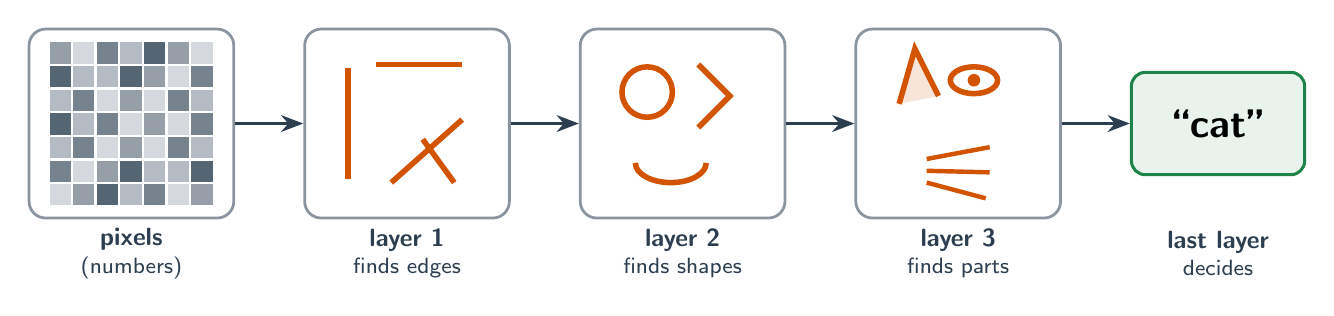
\begin{tikzpicture}[
  stage/.style={draw=ink!55, fill=white, rounded corners=6pt, line width=1pt, minimum width=2.6cm, minimum height=2.4cm},
  caption/.style={font=\small\bfseries, text=ink, align=center},
]
% Layers in a vision network: each layer builds on the one before.
\node[stage] (p) at (0,0) {};
\foreach \x in {-0.9,-0.6,...,0.9} \foreach \y in {-0.9,-0.6,...,0.9} {
  \pgfmathsetmacro{\g}{mod(int(abs(\x*10+\y*7)),5)*15+20}
  \fill[ink!\g] (\x-0.14,\y-0.14) rectangle ++(0.27,0.27);
}
\node[caption] at (0,-1.65) {pixels\\[-1pt]{\footnotesize\mdseries (numbers)}};

\node[stage] (e) at (3.5,0) {};
\draw[machine, line width=2pt] (2.75,-0.7) -- (2.75,0.7);
\draw[machine, line width=2pt] (3.1,0.75) -- (4.2,0.75);
\draw[machine, line width=2pt] (3.3,-0.75) -- (4.2,0.05);
\draw[machine, line width=2pt] (3.7,-0.2) -- (4.1,-0.75);
\node[caption] at (3.5,-1.65) {layer 1\\[-1pt]{\footnotesize\mdseries finds edges}};

\node[stage] (s) at (7,0) {};
\draw[machine, line width=2pt] (6.55,0.4) circle (0.32);
\draw[machine, line width=2pt] (7.2,0.75) -- (7.6,0.35) -- (7.2,-0.05);
\draw[machine, line width=2pt] (6.4,-0.5) arc (180:360:0.45 and 0.25);
\node[caption] at (7,-1.65) {layer 2\\[-1pt]{\footnotesize\mdseries finds shapes}};

\node[stage] (t) at (10.5,0) {};
% ear, eye, whiskers
\draw[machine, line width=2pt, fill=machine!15] (9.75,0.25) -- (9.95,0.95) -- (10.25,0.35);
\draw[machine, line width=2pt] (10.7,0.55) ellipse (0.3 and 0.17); \fill[machine] (10.7,0.55) circle (0.08);
\draw[machine, line width=1.6pt] (10.1,-0.45) -- (10.9,-0.3) (10.1,-0.6) -- (10.9,-0.62) (10.1,-0.75) -- (10.85,-0.95);
\node[caption] at (10.5,-1.65) {layer 3\\[-1pt]{\footnotesize\mdseries finds parts}};

\node[resultbox, font=\Large\bfseries, minimum width=2.2cm, minimum height=1.3cm] (o) at (13.8,0) {``cat''};
\node[caption] at (13.8,-1.65) {last layer\\[-1pt]{\footnotesize\mdseries decides}};
\draw[flow] (p) -- (e); \draw[flow] (e) -- (s); \draw[flow] (s) -- (t); \draw[flow] (t) -- (o);
\end{tikzpicture}
\end{document}
